\section{lg\-Tag Class Reference}
\label{classlgTag}\index{lgTag@{lgTag}}
GUIDO tag with name and a list of arguments given as {\bf lg\-Tag\-Arg}.  


{\tt \#include $<$lgtag.h$>$}

Inheritance diagram for lg\-Tag::\begin{figure}[H]
\begin{center}
\leavevmode
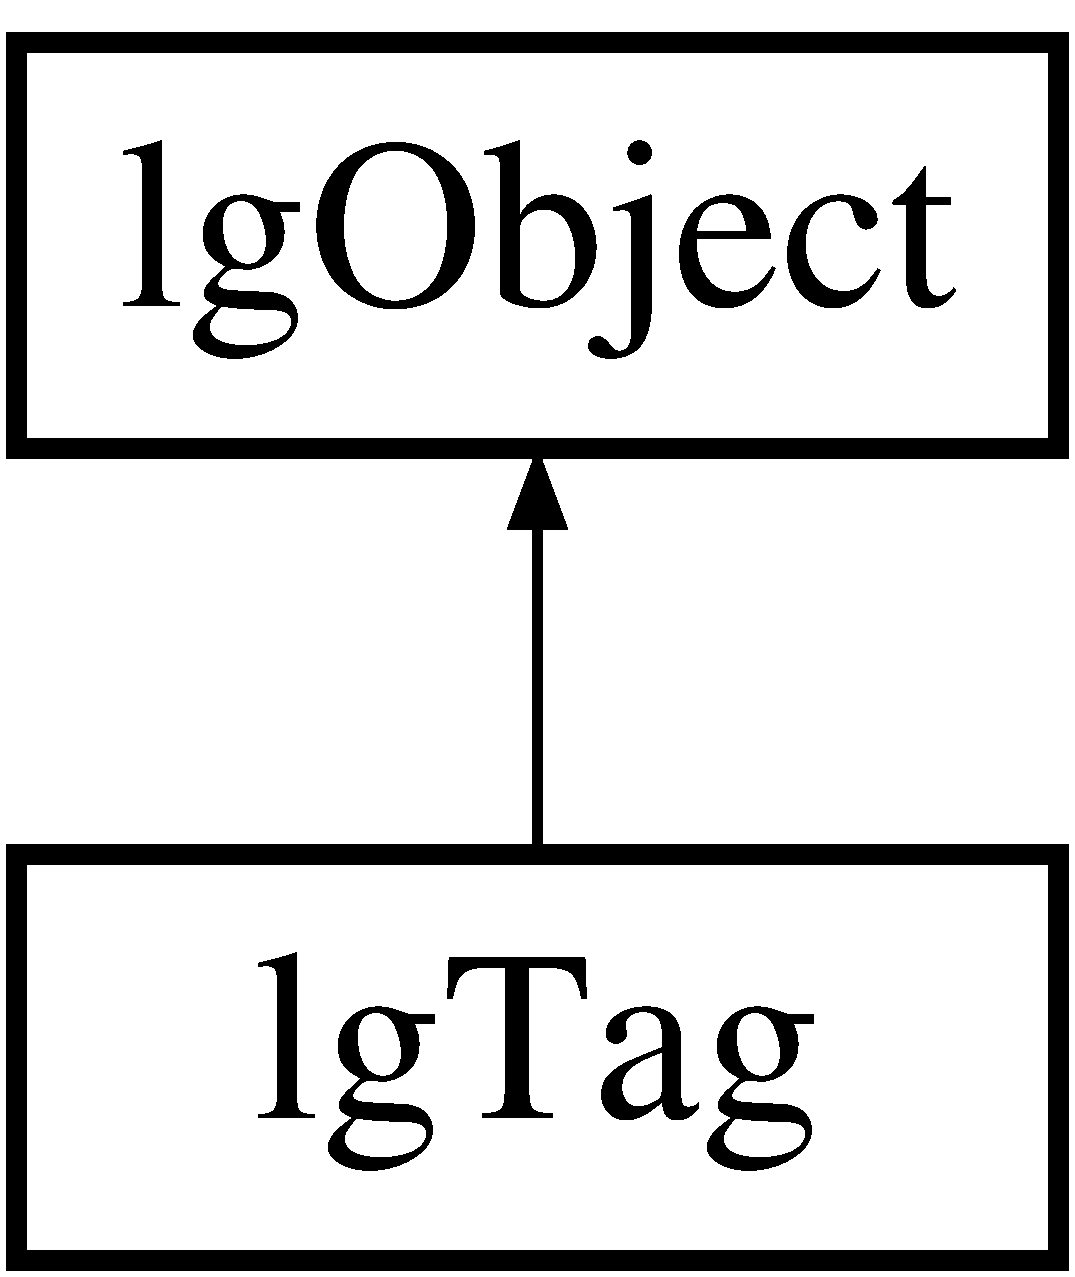
\includegraphics[height=2cm]{classlgTag}
\end{center}
\end{figure}
\subsection*{Public Member Functions}
\begin{CompactItemize}
\item 
int {\bf tag\-Type} (void)
\item 
int {\bf get\-Param\-Char} (const char $\ast$pname, int def\-Pos, string \&value, string \&unit)
\begin{CompactList}\small\item\em get parameter value as a string, return 0 if parameter does not exist \item\end{CompactList}\item 
int {\bf get\-Param\-Int} (const char $\ast$pname, int def\-Pos, int \&value, string \&unit)
\begin{CompactList}\small\item\em get parameter value as an int, return 0 if parameter does not exist \item\end{CompactList}\item 
int {\bf get\-Param\-Float} (const char $\ast$pname, int def\-Pos, double \&value, string \&unit)
\begin{CompactList}\small\item\em get parameter value as a double, return 0 if parameter does not exist \item\end{CompactList}\item 
void {\bf accept} ({\bf string\-Visitor} v)
\begin{CompactList}\small\item\em prototype, not used at the moment \item\end{CompactList}\item 
virtual string {\bf to\-String} ({\bf lg\-Voice} $\ast$v=NULL)
\begin{CompactList}\small\item\em convert tag and arguments into a string, add a range open \char`\"{}(\char`\"{} if needed \item\end{CompactList}\item 
string {\bf name} (void)
\item 
void {\bf set\-Name} (const char $\ast$str, const char $\ast$str2=NULL)
\item 
{\bf lg\-Tag} (long int id, {\bf lg\-Event} $\ast$p\-Ev, const char $\ast${\bf name\-I})
\begin{CompactList}\small\item\em create a new tag \item\end{CompactList}\item 
virtual {\bf $\sim$lg\-Tag} (void)
\item 
long int {\bf id} (void)
\begin{CompactList}\small\item\em unique tag id generated by the parser or given by user \item\end{CompactList}\item 
int {\bf c\-Args} (void)
\begin{CompactList}\small\item\em number of args \item\end{CompactList}\item 
{\bf lg\-Tag\-Arg} $\ast$ {\bf first\-Arg} (void)
\item 
{\bf lg\-Tag\-Arg} $\ast$ {\bf find\-Arg} (const char $\ast$name, int def\-Pos=0)
\begin{CompactList}\small\item\em search forargument by name, if not exists and def\-Pos $>$ -1 search at def\-Pos \item\end{CompactList}\item 
{\bf lg\-Tag\-Arg} $\ast$ {\bf get\-Arg} (int id)
\begin{CompactList}\small\item\em get tag arg 1...n \item\end{CompactList}\item 
void {\bf add\-Arg} ({\bf lg\-Tag\-Arg} $\ast$pa)
\begin{CompactList}\small\item\em add argument \item\end{CompactList}\item 
void {\bf remove\-Arg} ({\bf lg\-Tag\-Arg} $\ast$pa)
\begin{CompactList}\small\item\em remove arguemnt \item\end{CompactList}\item 
{\bf lg\-Event} $\ast$ {\bf p\-Event} (void)
\begin{CompactList}\small\item\em get event before tag, points to {\bf lg\-Sequence} at begin of sequence!! \item\end{CompactList}\item 
{\bf lg\-Event} $\ast$ {\bf first\-In\-Range} (void)
\begin{CompactList}\small\item\em get first event in range \item\end{CompactList}\item 
{\bf lg\-Event} $\ast$ {\bf last\-In\-Range} (void)
\begin{CompactList}\small\item\em get last event in range \item\end{CompactList}\item 
void {\bf set\-Range} ({\bf lg\-Tag} $\ast$ta)
\begin{CompactList}\small\item\em set a range by attavhing an \char`\"{})\char`\"{} or  tag \item\end{CompactList}\item 
{\bf lg\-Tag} $\ast$ {\bf end\-Range} (void)
\begin{CompactList}\small\item\em return end\-Range tag \char`\"{})\char`\"{} or \char`\"{}$\backslash$$\backslash$tag\-End\char`\"{} \item\end{CompactList}\item 
char {\bf has\-Range} (void)
\begin{CompactList}\small\item\em 1 if explicite range has been set \item\end{CompactList}\item 
char {\bf empty\-Range} (void)
\begin{CompactList}\small\item\em true if has\-Range and no notes inside! \item\end{CompactList}\item 
int {\bf split\-Range} (void)
\begin{CompactList}\small\item\em split (...) into   if tag has a range, and return 1 if range has been converted \item\end{CompactList}\item 
virtual lg\-Frac {\bf pos} (void)
\begin{CompactList}\small\item\em == prev\-I-$>$Attack + prev\-Ev-$>$Dur \item\end{CompactList}\item 
lg\-Frac {\bf end\-Pos} (void)
\begin{CompactList}\small\item\em result $<$ 0 if no range, please see readme.txt for issues \item\end{CompactList}\end{CompactItemize}
\subsection*{Private Attributes}
\begin{CompactItemize}
\item 
string {\bf name\-I}
\begin{CompactList}\small\item\em tag name including \char`\"{}$\backslash$\char`\"{} \item\end{CompactList}\item 
long int {\bf id\-I}
\begin{CompactList}\small\item\em unique id given by parser, end range tags have -1 $\ast$ startrange-$>$id \item\end{CompactList}\item 
{\bf lg\-Tag\-Arg} $\ast$ {\bf args\-I}
\begin{CompactList}\small\item\em list of arguments \item\end{CompactList}\item 
{\bf lg\-Event} $\ast$ {\bf prev\-Ev\-I}
\begin{CompactList}\small\item\em pointer to previous event, tag-range starts AFTER prev\-Ev\-I, is NULL if tag starts before first note of sequence! \item\end{CompactList}\item 
{\bf lg\-Tag} $\ast$ {\bf range\-End}
\begin{CompactList}\small\item\em pointer to close range tag \char`\"{})\char`\"{} or  \item\end{CompactList}\end{CompactItemize}
\subsection*{Friends}
\begin{CompactItemize}
\item 
class {\bf lg\-Chord}
\item 
class {\bf lg\-Voice}
\end{CompactItemize}


\subsection{Detailed Description}
GUIDO tag with name and a list of arguments given as {\bf lg\-Tag\-Arg}. 



\subsection{Constructor \& Destructor Documentation}
\index{lgTag@{lg\-Tag}!lgTag@{lgTag}}
\index{lgTag@{lgTag}!lgTag@{lg\-Tag}}
\subsubsection{\setlength{\rightskip}{0pt plus 5cm}lg\-Tag::lg\-Tag (long int {\em id}, {\bf lg\-Event} $\ast$ {\em p\-Ev}, const char $\ast$ {\em name\-I})}\label{classlgTag_a8}


create a new tag 

\begin{Desc}
\item[Parameters: ]\par
\begin{description}
\item[{\em 
id}]unique id \item[{\em 
p\-Ev}]previous event -$>$ time position of tag, if timepos == 0 -$>$ p\-Ev == {\bf lg\-Voice} \end{description}
\end{Desc}
\index{lgTag@{lg\-Tag}!~lgTag@{$\sim$lgTag}}
\index{~lgTag@{$\sim$lgTag}!lgTag@{lg\-Tag}}
\subsubsection{\setlength{\rightskip}{0pt plus 5cm}lg\-Tag::$\sim${\bf lg\-Tag} (void)\hspace{0.3cm}{\tt  [virtual]}}\label{classlgTag_a9}




\subsection{Member Function Documentation}
\index{lgTag@{lg\-Tag}!accept@{accept}}
\index{accept@{accept}!lgTag@{lg\-Tag}}
\subsubsection{\setlength{\rightskip}{0pt plus 5cm}void lg\-Tag::accept ({\bf string\-Visitor} {\em v})\hspace{0.3cm}{\tt  [inline]}}\label{classlgTag_a4}


prototype, not used at the moment 



Reimplemented from {\bf lg\-Object} {\rm (p.\,\pageref{classlgObject_a0})}.\index{lgTag@{lg\-Tag}!addArg@{addArg}}
\index{addArg@{addArg}!lgTag@{lg\-Tag}}
\subsubsection{\setlength{\rightskip}{0pt plus 5cm}void lg\-Tag::add\-Arg ({\bf lg\-Tag\-Arg} $\ast$ {\em pa})}\label{classlgTag_a15}


add argument 

\index{lgTag@{lg\-Tag}!cArgs@{cArgs}}
\index{cArgs@{cArgs}!lgTag@{lg\-Tag}}
\subsubsection{\setlength{\rightskip}{0pt plus 5cm}int lg\-Tag::c\-Args (void)}\label{classlgTag_a11}


number of args 

\index{lgTag@{lg\-Tag}!emptyRange@{emptyRange}}
\index{emptyRange@{emptyRange}!lgTag@{lg\-Tag}}
\subsubsection{\setlength{\rightskip}{0pt plus 5cm}char lg\-Tag::empty\-Range (void)}\label{classlgTag_a23}


true if has\-Range and no notes inside! 

\index{lgTag@{lg\-Tag}!endPos@{endPos}}
\index{endPos@{endPos}!lgTag@{lg\-Tag}}
\subsubsection{\setlength{\rightskip}{0pt plus 5cm}lg\-Frac lg\-Tag::end\-Pos (void)}\label{classlgTag_a26}


result $<$ 0 if no range, please see readme.txt for issues 

\index{lgTag@{lg\-Tag}!endRange@{endRange}}
\index{endRange@{endRange}!lgTag@{lg\-Tag}}
\subsubsection{\setlength{\rightskip}{0pt plus 5cm}{\bf lg\-Tag}$\ast$ lg\-Tag::end\-Range (void)\hspace{0.3cm}{\tt  [inline]}}\label{classlgTag_a21}


return end\-Range tag \char`\"{})\char`\"{} or \char`\"{}$\backslash$$\backslash$tag\-End\char`\"{} 

\index{lgTag@{lg\-Tag}!findArg@{findArg}}
\index{findArg@{findArg}!lgTag@{lg\-Tag}}
\subsubsection{\setlength{\rightskip}{0pt plus 5cm}{\bf lg\-Tag\-Arg} $\ast$ lg\-Tag::find\-Arg (const char $\ast$ {\em name}, int {\em def\-Pos} = 0)}\label{classlgTag_a13}


search forargument by name, if not exists and def\-Pos $>$ -1 search at def\-Pos 

\begin{Desc}
\item[Parameters: ]\par
\begin{description}
\item[{\em 
def\-Pos}]1...n \end{description}
\end{Desc}
\index{lgTag@{lg\-Tag}!firstArg@{firstArg}}
\index{firstArg@{firstArg}!lgTag@{lg\-Tag}}
\subsubsection{\setlength{\rightskip}{0pt plus 5cm}{\bf lg\-Tag\-Arg} $\ast$ lg\-Tag::first\-Arg (void)}\label{classlgTag_a12}


\index{lgTag@{lg\-Tag}!firstInRange@{firstInRange}}
\index{firstInRange@{firstInRange}!lgTag@{lg\-Tag}}
\subsubsection{\setlength{\rightskip}{0pt plus 5cm}{\bf lg\-Event} $\ast$ lg\-Tag::first\-In\-Range (void)}\label{classlgTag_a18}


get first event in range 

tag range starts at beginning of sequence \index{lgTag@{lg\-Tag}!getArg@{getArg}}
\index{getArg@{getArg}!lgTag@{lg\-Tag}}
\subsubsection{\setlength{\rightskip}{0pt plus 5cm}{\bf lg\-Tag\-Arg} $\ast$ lg\-Tag::get\-Arg (int {\em id})}\label{classlgTag_a14}


get tag arg 1...n 

\begin{Desc}
\item[Parameters: ]\par
\begin{description}
\item[{\em 
id}]1...n \end{description}
\end{Desc}
\index{lgTag@{lg\-Tag}!getParamChar@{getParamChar}}
\index{getParamChar@{getParamChar}!lgTag@{lg\-Tag}}
\subsubsection{\setlength{\rightskip}{0pt plus 5cm}int lg\-Tag::get\-Param\-Char (const char $\ast$ {\em pname}, int {\em def\-Pos}, string \& {\em value}, string \& {\em unit})}\label{classlgTag_a1}


get parameter value as a string, return 0 if parameter does not exist 

\begin{Desc}
\item[Parameters: ]\par
\begin{description}
\item[{\em 
pname}]parameter name (might be NULL) \item[{\em 
def\-Pos}]default position of paramter 1...n \item[{\em 
value}]value \item[{\em 
unit}]unit if available \end{description}
\end{Desc}
\index{lgTag@{lg\-Tag}!getParamFloat@{getParamFloat}}
\index{getParamFloat@{getParamFloat}!lgTag@{lg\-Tag}}
\subsubsection{\setlength{\rightskip}{0pt plus 5cm}int lg\-Tag::get\-Param\-Float (const char $\ast$ {\em pname}, int {\em def\-Pos}, double \& {\em value}, string \& {\em unit})}\label{classlgTag_a3}


get parameter value as a double, return 0 if parameter does not exist 

\begin{Desc}
\item[Parameters: ]\par
\begin{description}
\item[{\em 
pname}]parameter name (might be NULL) \item[{\em 
def\-Pos}]default position of paramter, 1...n \item[{\em 
value}]value \item[{\em 
unit}]unit if available \end{description}
\end{Desc}
\index{lgTag@{lg\-Tag}!getParamInt@{getParamInt}}
\index{getParamInt@{getParamInt}!lgTag@{lg\-Tag}}
\subsubsection{\setlength{\rightskip}{0pt plus 5cm}int lg\-Tag::get\-Param\-Int (const char $\ast$ {\em pname}, int {\em def\-Pos}, int \& {\em value}, string \& {\em unit})}\label{classlgTag_a2}


get parameter value as an int, return 0 if parameter does not exist 

\begin{Desc}
\item[Parameters: ]\par
\begin{description}
\item[{\em 
pname}]parameter name (might be NULL) \item[{\em 
def\-Pos}]default position of paramter, 1...n \item[{\em 
value}]value \item[{\em 
unit}]unit if available \end{description}
\end{Desc}
\index{lgTag@{lg\-Tag}!hasRange@{hasRange}}
\index{hasRange@{hasRange}!lgTag@{lg\-Tag}}
\subsubsection{\setlength{\rightskip}{0pt plus 5cm}char lg\-Tag::has\-Range (void)}\label{classlgTag_a22}


1 if explicite range has been set 

\index{lgTag@{lg\-Tag}!id@{id}}
\index{id@{id}!lgTag@{lg\-Tag}}
\subsubsection{\setlength{\rightskip}{0pt plus 5cm}long int lg\-Tag::id (void)\hspace{0.3cm}{\tt  [inline]}}\label{classlgTag_a10}


unique tag id generated by the parser or given by user 

\index{lgTag@{lg\-Tag}!lastInRange@{lastInRange}}
\index{lastInRange@{lastInRange}!lgTag@{lg\-Tag}}
\subsubsection{\setlength{\rightskip}{0pt plus 5cm}{\bf lg\-Event} $\ast$ lg\-Tag::last\-In\-Range (void)}\label{classlgTag_a19}


get last event in range 

\index{lgTag@{lg\-Tag}!name@{name}}
\index{name@{name}!lgTag@{lg\-Tag}}
\subsubsection{\setlength{\rightskip}{0pt plus 5cm}string lg\-Tag::name (void)}\label{classlgTag_a6}


\index{lgTag@{lg\-Tag}!pEvent@{pEvent}}
\index{pEvent@{pEvent}!lgTag@{lg\-Tag}}
\subsubsection{\setlength{\rightskip}{0pt plus 5cm}{\bf lg\-Event}$\ast$ lg\-Tag::p\-Event (void)\hspace{0.3cm}{\tt  [inline]}}\label{classlgTag_a17}


get event before tag, points to {\bf lg\-Sequence} at begin of sequence!! 

\index{lgTag@{lg\-Tag}!pos@{pos}}
\index{pos@{pos}!lgTag@{lg\-Tag}}
\subsubsection{\setlength{\rightskip}{0pt plus 5cm}lg\-Frac lg\-Tag::pos (void)\hspace{0.3cm}{\tt  [virtual]}}\label{classlgTag_a25}


== prev\-I-$>$Attack + prev\-Ev-$>$Dur 

check an event before the tag

the tag is first tag in voice 

Reimplemented from {\bf lg\-Object} {\rm (p.\,\pageref{classlgObject_a5})}.\index{lgTag@{lg\-Tag}!removeArg@{removeArg}}
\index{removeArg@{removeArg}!lgTag@{lg\-Tag}}
\subsubsection{\setlength{\rightskip}{0pt plus 5cm}void lg\-Tag::remove\-Arg ({\bf lg\-Tag\-Arg} $\ast$ {\em pa})}\label{classlgTag_a16}


remove arguemnt 

\index{lgTag@{lg\-Tag}!setName@{setName}}
\index{setName@{setName}!lgTag@{lg\-Tag}}
\subsubsection{\setlength{\rightskip}{0pt plus 5cm}void lg\-Tag::set\-Name (const char $\ast$ {\em str}, const char $\ast$ {\em str2} = NULL)\hspace{0.3cm}{\tt  [inline]}}\label{classlgTag_a7}


\begin{Desc}
\item[Parameters: ]\par
\begin{description}
\item[{\em 
str}]neq name of this \item[{\em 
str2}]name of end range tag \end{description}
\end{Desc}
\index{lgTag@{lg\-Tag}!setRange@{setRange}}
\index{setRange@{setRange}!lgTag@{lg\-Tag}}
\subsubsection{\setlength{\rightskip}{0pt plus 5cm}void lg\-Tag::set\-Range ({\bf lg\-Tag} $\ast$ {\em ta})}\label{classlgTag_a20}


set a range by attavhing an \char`\"{})\char`\"{} or  tag 

\index{lgTag@{lg\-Tag}!splitRange@{splitRange}}
\index{splitRange@{splitRange}!lgTag@{lg\-Tag}}
\subsubsection{\setlength{\rightskip}{0pt plus 5cm}int lg\-Tag::split\-Range (void)}\label{classlgTag_a24}


split (...) into   if tag has a range, and return 1 if range has been converted 

split (..) ranges into   ranges if the last\-In\-Range and prev\-Ev events are located in different voices (should never happen) the $\backslash$...end should be placed in the voice of last\-In\-Range! \index{lgTag@{lg\-Tag}!tagType@{tagType}}
\index{tagType@{tagType}!lgTag@{lg\-Tag}}
\subsubsection{\setlength{\rightskip}{0pt plus 5cm}int lg\-Tag::tag\-Type (void)}\label{classlgTag_a0}


\index{lgTag@{lg\-Tag}!toString@{toString}}
\index{toString@{toString}!lgTag@{lg\-Tag}}
\subsubsection{\setlength{\rightskip}{0pt plus 5cm}string lg\-Tag::to\-String ({\bf lg\-Voice} $\ast$ {\em v} = NULL)\hspace{0.3cm}{\tt  [virtual]}}\label{classlgTag_a5}


convert tag and arguments into a string, add a range open \char`\"{}(\char`\"{} if needed 



Reimplemented from {\bf lg\-Object} {\rm (p.\,\pageref{classlgObject_a3})}.

\subsection{Friends And Related Function Documentation}
\index{lgTag@{lg\-Tag}!lgChord@{lgChord}}
\index{lgChord@{lgChord}!lgTag@{lg\-Tag}}
\subsubsection{\setlength{\rightskip}{0pt plus 5cm}friend class {\bf lg\-Chord}\hspace{0.3cm}{\tt  [friend]}}\label{classlgTag_n0}




Reimplemented from {\bf lg\-Object} {\rm (p.\,\pageref{classlgObject_n5})}.\index{lgTag@{lg\-Tag}!lgVoice@{lgVoice}}
\index{lgVoice@{lgVoice}!lgTag@{lg\-Tag}}
\subsubsection{\setlength{\rightskip}{0pt plus 5cm}friend class {\bf lg\-Voice}\hspace{0.3cm}{\tt  [friend]}}\label{classlgTag_n1}




Reimplemented from {\bf lg\-Object} {\rm (p.\,\pageref{classlgObject_n1})}.

\subsection{Member Data Documentation}
\index{lgTag@{lg\-Tag}!argsI@{argsI}}
\index{argsI@{argsI}!lgTag@{lg\-Tag}}
\subsubsection{\setlength{\rightskip}{0pt plus 5cm}{\bf lg\-Tag\-Arg}$\ast$ {\bf lg\-Tag::args\-I}\hspace{0.3cm}{\tt  [private]}}\label{classlgTag_r2}


list of arguments 

\index{lgTag@{lg\-Tag}!idI@{idI}}
\index{idI@{idI}!lgTag@{lg\-Tag}}
\subsubsection{\setlength{\rightskip}{0pt plus 5cm}long int {\bf lg\-Tag::id\-I}\hspace{0.3cm}{\tt  [private]}}\label{classlgTag_r1}


unique id given by parser, end range tags have -1 $\ast$ startrange-$>$id 

\index{lgTag@{lg\-Tag}!nameI@{nameI}}
\index{nameI@{nameI}!lgTag@{lg\-Tag}}
\subsubsection{\setlength{\rightskip}{0pt plus 5cm}string {\bf lg\-Tag::name\-I}\hspace{0.3cm}{\tt  [private]}}\label{classlgTag_r0}


tag name including \char`\"{}$\backslash$\char`\"{} 

\index{lgTag@{lg\-Tag}!prevEvI@{prevEvI}}
\index{prevEvI@{prevEvI}!lgTag@{lg\-Tag}}
\subsubsection{\setlength{\rightskip}{0pt plus 5cm}{\bf lg\-Event}$\ast$ {\bf lg\-Tag::prev\-Ev\-I}\hspace{0.3cm}{\tt  [private]}}\label{classlgTag_r3}


pointer to previous event, tag-range starts AFTER prev\-Ev\-I, is NULL if tag starts before first note of sequence! 

\index{lgTag@{lg\-Tag}!rangeEnd@{rangeEnd}}
\index{rangeEnd@{rangeEnd}!lgTag@{lg\-Tag}}
\subsubsection{\setlength{\rightskip}{0pt plus 5cm}{\bf lg\-Tag}$\ast$ {\bf lg\-Tag::range\-End}\hspace{0.3cm}{\tt  [private]}}\label{classlgTag_r4}


pointer to close range tag \char`\"{})\char`\"{} or  



The documentation for this class was generated from the following files:\begin{CompactItemize}
\item 
{\bf lgtag.h}\item 
{\bf lgtag.cpp}\end{CompactItemize}
